%!TeX program=pdflatex
%!TeX encoding=utf8
%!TeX spellcheck = en_US
%!TeX root = ../../messageVortex.tex

\partepigraph{No matter how hard you work, someone else is working harder.}{Elon Musk, entrepreneur}
\part{Implementation\label{sec:implementation}}
The implementation differs from the academic model in some details. It is formeost more precise than the academic model. Furthermore, it requires a strict definition of the implementation in order to guarantee the interoperability between different implementations.

This section focuses therefore on the details of the reference implementation.

\chapter{Selection of Algorithms, Encodings, and Protocols}
In this chapter, we choose the following mandatory supported algorithms:
\begin{itemize}
	\item Encoding: ASN.1
	\item Encryption
	\begin{itemize}
		\item AES128/256
		\item Camellia128/256
	\end{itemize}
    \item Modes
    \begin{itemize}
    	\item ECB
    	\item GCM
    \end{itemize}
	\item Paddings
	\begin{itemize}
		\item PKCS\#1
		\item PKCS\#7
	\end{itemize}
	\item MACs
	\begin{itemize}
		\item SHA256/512
		\item RIPE-MD256
	\end{itemize}
	\item PRNG
	\begin{itemize}
		\item mrg32k3a
		\item blumMicali
	\end{itemize}
\end{itemize}

Where security relevant we always choose two independent algorithms. As our protocol has the means of signaling them, we may support additional algorithms without affecting communication while improving the variety of available algorithms.

In the following sections, we emphasize on the choice and the encoding used on the protocol level.

For all algorithms we apply the following criteria:
\begin{itemize}
	\item Always focus on common standards
	\item Focus on interoperability when selecting standards
	\item Focus on efficiency (wherever possible use simple, parallelizable algorithms)
	\item When sensible and possible chose at least two unrelated algorithms (e.g., cryptographic algorithms or MACs)
\end{itemize}

\fxwarning{Sumarize subsections}

\section{Encoding Scheme}
As encoding scheme we specified ASN.1\cite{dis19878824}. It is more compact than the originally selected XML-Standard. It is very common in the fields of telecommunication and encryption (e.g. X509 certificates are represented in ASN.1). To maintain biggestmost interoperability, we choose DER encoding as it has exactly one possible representation for every value. This is especially important when dong signing or solving puzzles in our case.

On the downside ASN-1 encoding is, unlike XML, not human readable. As we hide the messages anyway, we considered this as minor flaw, as we need to have an extracting program anyway to see the content of a message.

\section{Cipher Selection}
In this protocol, a lot of encryption and hashing algorithms have to be used. This choice of these algorithms should be explained. 

We decided to define fixed key sizes for symmetric ciphers as we went with block ciphres. For the asymmetric ciphres we encode the keysize in the parameters as they are due to their differences far more often flexible.

\begin{figure}[ht]
\lstinputlisting[linerange={6-100},language=asn.1,multicols=2]{../../../../application-core-library/src/main/asn/MessageVortex-Ciphers.asn}
\caption{Definition of the structures related to ciphers}
\label{fig:defCiphers}
\end{figure}

From the requirements side, we have to follow the following principle:
First of all, we need a subset of encryption algorithms all implementations may rely on. Defining such a subset guarantees interoperability between all nodes regardless of their origins. 

Secondly, we need to have a spectrum of algorithms in such a manner that it may be (a) enlarged if necessary and (b) there is an alternative if an algorithm (or a mathematical problem class) is broken (so that algorithms may be withdrawn if required without affecting the function in general). 

And third, due to the onion-like design described in this document, asymmetric encryption should be avoided in favor of symmetric encryption to minimize losses due to the key length and the generally higher CPU load opposed by asymmetric keys.

If the algorithm is generally bound to specific key sizes (due to S-Boxes or similar constructs), the key size is incorporated into the definition. If not, the key size is handled as a parameter.

The key sizes have been chosen in such a manner that the key types form tuples of approximately equal strength. The support of Camelia192 and Aes192 has been defined as optional. However, as they are wildly common in implementations, they have already been standardized as they build a possibility to step up security in the future.

Having these criteria for choice, we chose to use the following keys and key sizes:
\begin{itemize}
	\item Symmetric
	\begin{itemize}
		\item AES (key sizes: 128, 192, 256)
		\item Camellia (key sizes: 128, 192, and 256)
	\end{itemize}
	\item Asymmetric
	\begin{itemize}
		\item RSA (key size: 2048, 4096, and 8192)
		\item Named Elliptic Curves
		\begin{itemize}
			\item secp384r1
			\item sect409k1
			\item secp521r1
		\end{itemize}
	\end{itemize}
	\item Hashing
	\begin{itemize}
		\item sha3-256
		\item sha3-384
		\item sha3-512
		\item RIPE-MD160
		\item RIPE-MD256
		\item RIPE-MD320
	\end{itemize}
\end{itemize}

Within the implementation, we assigned algorithms to a security strength level:
\begin{itemize}
	\item LOW\\
	AES128, Camellia128, RSA1024, sha3-256
	\item MEDIUM\\
	AES192, Camellia 192, RSA2048, ECC secp384r1, sha3-256
	\item HIGH\\
	AES256, Camellia256, RSA4096, ECC sect409k1, sha3-384
	\item QUANTUM\\
	AES256, Camellia256, RSA8192, ECC secp521r1, ntru, sha3-512
\end{itemize}

This allows categorizing the used algorithms to a strength. This list, however, should only serve the purpose of selecting algorithms for people without cryptological know-how.

\section{Mode Selections}
We evaluated the most common cipher modes for suitability. For MessageVortex, we focussed on modes that have the properties parallelizable, random access, and do not do authentication. The main focus, besides the characteristics mentioned before, was on the question of whether there is an open implementation available in java, which is reasonably tested.

\begin{figure}[ht]
	\lstinputlisting[linerange={99-112},language=asn.1]{../../../../application-core-library/src/main/asn/MessageVortex-Ciphers.asn}
	\caption{Enumeration definition of modes in ASN.1 with support requirements.}
	\label{fig:defModes}
\end{figure}

Figure~\ref{fig:defModes} shows the selected paddings and their requirement level.

Very important was, that we quite often reencrypt already encrypted content. As a result we had not to exclude algorithms such as ECB.

\begin{itemize}
	\item ECB (Electronic Code Book)\\
	      ECB is the most basic mode. Each block of the cleartext is encrypted on its own. This results in a big flaw: blocks containing the same data will always transform to the same ciphertext. This property makes it possible to see some structures of the plain text when looking at the ciphertext. This solution allows the parallelization of encryption, decryption, and random access while decrypting. Due to these flaws, we rejected this mode.
	\item CBC (Cypher Block Chaining)\\  
	      CBC extends the encryption by xor'ing an initialization vector into the first block before encrypting. For all subsequent blocks, the ciphertext result of the preceding block is taken as xor input. This solution does not allow parallelization of encryption, but decryption may be paralleled, and random access is possible. As another downside, CBC requires a shared initialization vector. As with most IV bound modes, an IV/key pair should not be used twice, which has implications for our protocol.
	\item PCBC (Propagation Cypher Block Chaining)\\
	      CBC extends the encryption by xor'ing, not the ciphertext but a xor result of ciphertext and plaintext. This modification denies parallel decryption and random access compared to CBC.
	\item EAX\\      
	      EAX has been broken in 2012\cite{minematsu2013attacks} and is therefore rejected for our use.
	\item CFB (Cypher Feedback)
	      CFB is specified in \cite{dworkin2001recommendation} and works precisely as CBC with the difference that the plain text is xor'ed and the initialization vector, or the preceding cipher result is encrypted. CFB does not support parallel encryption as the ciphertext input from the preceding operation is required for an encryption round. CFB does, however, allow parallel decryption and random access.
	\item OFB\\
	      \cite{dworkin2001recommendation} specifies OFB and works exactly as CFB except for the fact that not the ciphertext result is taken as feedback but the result of the encryption before xor'ing the plain text. This denies parallel encryption and decryption, as well as random access.
	\item OCB (Offset Codebook Mode)\\
	      This mode was first proposed in \cite{rogaway2003ocb} and later specified in \cite{krovetz-ocb-04}. OCB is specifically designed for AES128, AES192, and AES256. It supports authentication tag lengths of 128, 96, or 64 bits for each specified encryption algorithm. OCB hashes the plaintext of a message with a specialized function $H_{OCB}(\mathbf{M})$. OCB is fully parallelizable due to its internal structure. All blocks except the first and the last can be encrypted or decrypted in parallel.
	\item CTR\\
	      CTR is specified in \cite{lipmaa2000ctr} and is a mixture between OFB and CBC. A nonce concatenated with a counter incrementing on every block is encrypted and then xor'ed with the plain text. This mode allows parallel decryption and encryption, as well as random access. Reusing IV/Key-pairs using CTR is a problem as we might derive the xor'ed product of two messages. This problem only applies where messages are not uniformly random such as in an already encrypted block.
	\item CCM\\
	      Counter with CBC-MAC (CCM) is specified in \cite{RFC3610}. It allows to pad and authenticate encrypted and unencrypted data. It furthermore requires a nonce for its operation. The size of the nonce is dependent on the number of octets in the length field. In the first 16 bytes of the message, the nonce and the message size is stored. For the encryption itself, CTR is used. It shares the same properties as CTR. 
	
	      It allows parallel decryption and encryption as well as random access.
	\item GCM (Galois Counter Mode)\\
	      GCM has been defined in \cite{mcgrew2004galois}, and is related to CTR but has some major differences. The nonce is not used (just the counter starting with value 1). To authenticate the encryption, an authentication token $auth$ is hashed with $H_{GFmult}$ and then xor'ed with the first cipher block. All subsequent cipher blocks are xor'ed with the previous result and then hashed again with $H_{GFmult}$. After the last block the output $o$ is processed  as follows: $H_{GFmult}(o\bigoplus (len(A)||len(B))) \bigoplus E^{K^0}(counter_0)$. As a result, GCM is not parallelizable and does not support random access.
	
	      The mode has been analyzed security-wise in \citeyear{mcgrew2004security} and showed no weaknesses in the analyzed fields \cite{mcgrew2004security}. 
	
	      GCM supports parallel Encryption and decryption. Random access is possible. However, authentication of encryption is not parallelizable. The authentication makes it unsuitable for our purposes. Alternatively, we could use a fixed authentication string.
	\item XTS (XEX-based tweaked-codebook mode with ciphertext stealing)\\
	      This mode is standardized in IEEE 1619-2007 (soon to be superseded). A rough overview of XTS may be found at \cite{Martin2010}. It was developed initially for Disks offering random access and authentication at the same time. 
	\item CMC (CBC-mask-CBC) and EME (ECB-mask-ECB)\\ 
	      In \cite{Halevi:2003} \citeauthor{Halevi:2003} introduces a cipher mode which is extremely costly as it requires two encryptions. CMC is not parallelizable due to the underlying CBC mode, but EME is. 
	\item LRW\\
	      LRW is a tweakable narrow-block cipher mode described in \cite{tschorsch:translayeranon}. This mode shares the same properties as EBC but without the weakness of the same clear text block resulting in the same ciphertext. Similarly to XEX, it requires a tweak instead of an IV.
\end{itemize}

We decided to go with mainly cbc. However, most of the implementations are available and lightweight, we therefore were not as restrictive as ususal when defining a minimal set

\section{Padding selection}
A plain text stream may have any length. Since we always encrypt in blocks of a fixed size, we need a mechanism to indicate how many bytes of the last encrypted block may be safely discarded. 

We have chosen for the paddings outlined in figure~\ref{fig:defPaddings} to be supported.
\begin{figure}[ht]
	\lstinputlisting[linerange={114-121},language=asn.1]{../../../../application-core-library/src/main/asn/MessageVortex-Ciphers.asn}
	\caption{Enumeration definition of paddings in ASN.1 with support requirements.}
	\label{fig:defPaddings}
\end{figure}

\subsection{RSAES-PKCS1-v1\_5 and RSAES-OAEP}
This padding is the older of the paddings standardized for PKCS1. It is basically a prefix of two bytes followed by a padding set of non zero bytes and then terminated by a zero byte and then followed by the message. This padding may give a clue if decryption was successful or not. RSAES-OAEP ist the newer of the two padding standards 

\subsection{PKCS7} 
This padding is the standard used in many places when applying symmetric encryption up to 256 bits key length. The free bytes in the last cipher block indicate the number of bytes being used. This makes this padding very compact. It requires only 1 Byte of functional data at the end of the block. All other bytes are defined but not needed.

\subsection{OAEP with SHA and MGF1 padding} 
This padding is closely related to RSAES-OAEP padding. The hash size is, however, bigger, and thus, the required space for padding is much higher. OAEP with SHA and MGF1 Padding is used in asymmetric encryption only. Due to its size, it is important to note that the payload in the last block shrinks to $keySizeInBits/8-2-MacSize/4$.

In our approach, we have chosen to allow these four paddings. The allowed sha sizes match the allowed mac sizes chosen above. It is important to note that padding costs space at the end of a stream. Since we are always using one block for signing, we have to take care that the chosen signing mac plus the bytes required for padding do not exceed the key size of the asymmetric encryption. While this usually is not a problem for RSA as there are keys 1024+ Bits required, it is an essential problem for ECC algorithms as there are much shorter keys needed to achieve an equivalent strength compared to RSA. 

\subsection{Honorable Mention: AP Padding for $redundancy$ Operations}
We have introduced an additional type of padding not related to these paddings. We required for the $addRedundancy$ the following unique properties. Unfortunately, we were unable to find any padding which matched the following properties simultaneously:

\begin{itemize}
	\item Padding must not leak successful decryption\\
	      For our $addRedundancy$ operation, we required padding that had no detectable structure as a node should not be able to tell whether a $removeRedundancy$ operation did generate content or decoy. 
	\item Padding of more than one block\\
	Due to the nature of the operation, it is required to be able to pad more than just one block.
\end{itemize}

This padding is the only padding for the $addRedundancy$ and $removeRedundancy$ operations.

\subsection{Pseudo Random Number Generator Selection\label{sec:prng}}
For our $addRedundancy$ and $removeRedundancy$ operations we needed a pseudo random number generator (PRNG). For our implementation we did not research deeply this part as it seemed irrelevant. The only criteriion was, that it had to create content indistinguishable from an encrypted message. This criterion arose as we use it for padding invisibly an already encrypted message.

The PRNG used for our implementation is an xorshift+ generator. It is based on the XSadd PRNG\cite{marsaglia2003xorshift} and passes the bigcrush PRNG test suite. It is a fast, xor based PRNG which has two internal 64 bit seed states $s_0$ respectively $s_1$ and is defined as follows:

\begin{eqnarray}
x & = & s_0\\
s_0 & = & s_1\\
x & = & x \oplus ( x \ll 23 )\\
s_1 & = & x \oplus s_1 \oplus ( x \gg 17 ) \oplus (s_1 \gg 26 )\\
nextNumber & = & s_1+s_0
\end{eqnarray}

We have chosen this comparably weak PRNG for practical reasons. It is fast, simple, and is based on operations easy to implement on hardware. As we do not need a cryptographically strong PRNG, it is our primary choice so far. 

As the protocol is heavily dependent on security we have introduced everywhere at least one alternate algorithm which may be used if one of the choices may become a problem. In order to have a second choice for the PRNG we define the Blum-Micali PRNG as described in \cite{blum1984generate}. This PRNG is a cryptographically secure PRNG and is defined as follows:

$p$ is prime and $g$ is a primitive root modulo $p$. $x_0$ reflects the seed state.

\begin{eqnarray}
x_{i+1}=g^{x_i}\mod p
\end{eqnarray}

%\subsection{Puzzle Selection}
%\fxwarning{Add content here... maybe old text about PoW-Algorithms}
% Erradicated old text too inocomplete and massive work required

\section{Transport Layer Protocol Selection}
The following sections list common Internet protocols. We analyze those protocols for the fitness as transport layer of message vortex. 

We will identify SMTP and XMPP as good transport layer protocols for the \MessageVortex approach, as they have all required properties.

All sections are structured the same way. We first refer to the protocol or standard and describe it in the simplest possible form. We refer to subsequent standards if required to consider extensions where sensible. We then apply the previously referenced criteria and make a concise summary of the suiting of the protocol as a transport layer. The findings of this section is listed in table \ref{tab:protoSuitCrit}. The list here does not reflect the quality or maturity of the protocols. It is a simple analysis of suiting as a transport layer.

All sections are structured the same way. 
\begin{itemize}
	\item Description\\
	We first refer to the protocol or standard and describe it in the simplest possible form. We refer to subsequent standards if required to consider extensions where sensible.
	\item Apply criteria\\\\
	We then apply the previously referenced criteria and make a concise summary of the suiting of the protocol as a transport layer. The findings of this section is listed in table \ref{tab:protoSuitCrit}. The list here does not reflect the quality or maturity of the protocols. It is a simple analysis of suiting as a transport layer.
\end{itemize} 

\subsection{Applied Criteria\label{sec:transportCriteria}}
\begin{itemize}
	\item Widely adopted (Ct1)\\
	The more widely adopted and used a protocol is, the harder it is due to the sheer mass for an adversary to monitor , filter, or block the protocol. This is important for censorship resistance of the protocol. 
	\item Reliable (Ct2)\\
	Message transport between peers should be reliable. As messages may arrive anytime from everywhere, we do not have means to synchronize the peer partners on a higher level without investing a considerable effort. Furthermore, the availability of information when what type of information should be available at a specific point in the system would drastically simplify the identification of peers. To avoid synchronization, we do look for inherently reliable protocols.
	\item Symmetrical built (Ct3)\\
	The transport layer should rely on a peer to peer base. All servers implement a generic routing that requires no prior knowledge of all possible targets. This criterion neglects centralized infrastructures. This criterion may be dropped, assuming that the blending layer or a specialized transport overlay is responsible for routing.
\end{itemize}

\subsection{Analyzed Protocols}
We were unable to find a comprehensive list of protocols being used within the Internet and their bandwidth consumption. A weak reference is \cite{zhou2011examining}. This wekaness is founded in the fact that traffic in this report is callified among two critera: Know server or known port. As streaming services consume a considerable part of the Internet bandwidth (acording to the report more than 60\% download). The focus on the report lies on the bandwidth intense figures. However, leavin aside all sources which are strictly one way or dominated by a small number of companies worldwide, the ``top 10'' list of the report shrinks to the two categories ``File sharing'' (Rank 5; 4.2\% download and 30.2\% upload) and ``Messaging'' (Rank 8; 1.6\% download and 8.3\% upload bandwidth). 

In lack of such material we first collected a list of all common Internet messaging protocols (synchronous and asynchronous). We added furthermore some of the most common transfer protocols such as HTTP and FTP and analyzed this list.

\begin{itemize}
	\item Messaging Protocols
	\begin{itemize}
		\item SMTP
		\item CoAP
		\item MQTT
		\item AMQP
		\item XMPP
		\item WAMP
		\item SMS
		\item MMS
	\end{itemize}
	\item Other Protocols
	\begin{itemize}
		\item FTP, SFTP, and FTPS
		\item TFTP
		\item HTTP
	\end{itemize}
\end{itemize}

The following protocols have been discarded as we have considered them as outdated:
\begin{itemize}
	\item MTP\cite{RFC780} (obsoleted by SMTP)
	\item NNTP\cite{RFC3977} (outdated and has only a small usage acording to \cite{kim2010today})
\end{itemize}

We furthermore discarded all RPC-related protocols as they would by definition violate Ct3.

\subsection{Analysis}
\subsubsection{HTTP}
The HTTP protocol allows message transfer from and to a server and is specified in RFC2616 \cite{rfc2616}. It is not suitable as a communication protocol for messages due to the lack of notifications. There are some extensions that would allow such communications (such as WebDAV). Still, in general, even those are not suitable as they require a continuous connection to the server to get notifications. Having a ``rollup'' of notifications when connecting is not there by default but could be implemented on top of it. HTTP servers listen on standard ports 80 or 443 for incoming connects. The port 443 is equivalent to the port 80 except for the fact that it has a wrapping encryption layer (usually TLS). The incoming connects (requests) must offer a header part and may contain a body part that would be suitable for transferring messages to the server. The reply to this request is transferred over the same TCP connection containing the same two sections.

HTTP0.9-HTTP/1.1 are clear text protocols which are human-readable (except for the data part which might contain binary data). The HTTP/2\cite{rfc7540} protocol is using the same ports and default behavior. Unlike HTTP/0.9-HTTP/1.1, it is not a clear text but encodes headers and bodies in binary form. 

To be a valid candidate as storage, unauthenticated WebDAV support, as specified in \cite{rfc4918}, must be assumed.

The protocol does satisfy the first two main criteria (Ct1: Widely Adopted and Ct2: Reliable). The main disadvantage in terms of a message transport protocol is that this protocol is not symmetrically. A server is always just ``serving requests'' and not sending information actively to peers. This Request-Reply violates criteria (Ct3: Symmetrically built) and makes the protocol not a primary choice for message transport. 

It is possible to add such behavior to the blending layer using HTTP servers as pure storage. Such a behavior would however be most likely detectable and thus no longer be censorship resistant.

\subsubsection{FTP}
FTP is defined in RFC959\cite{RFC959}. This Protocol is intended for authenticated file transfer only. There is an account available for general access (``anonymous''). This account does normally not offer upload rights for security reasons. It is possible to use FTP as a message transfer endpoint. The configuration would work as follows: the user ``anonymous'' has upload rights only. It is unable to download or list a directory. A node may upload a message with a random name. In case a collision arises, the node retries with another random name. The blending layer picks messages up using an authenticated user. This workaround has multiple downsides. At first, handling FTP that way is very uncommon and usually requires an own dedicated infrastructure. Such beavior would make the protocol again possibly detectable. Secondly, passwords are always sent in the clear within FTP. Encryption as a wrapping layer (FTPS) is not common, and SFTP (actually a subsystem of SSH) has nothing in common with FTP except for the fact that it may transfer files as well.

Furthermore, FTP may be problematic when used in active mode for firewalls. All these problems make FTP not very suitable as a transport layer protocol. FTPS and SFTP feature similar weaknesses as the FTP version in terms of detectability of non-standard behavior.

Like in HTTP, a disadvantage of FTP in terms of a message transport protocol is that this protocol is not symmetrically. A server is always just ``serving requests'' and not sending information actively to peers. This Request-Reply violates criteria (Ct3: Symmetrically built) and makes the protocol not a primary choice for message transport. The Protocol, however, satisfies the first two criteria  (Ct1: Widely Adopted and Ct2: Reliable).

\subsubsection{TFTP}
TFTP has, despite its naming similarities to FTP, very little in common with it. TFTP is a UDP based file transfer protocol without any authentication scheme. The possibility of unauthenticated message access makes it not suitable as a transport layer. The protocol is due to the use of UDP in a meshed network with redundant routes. Since the Internet has a lot of these redundant routes, this neglects the use of this protocol.

TFTP is rarely ever used on the Internet, as its UDP based nature is not suitable for a network with redundant routes. Not being common on the Internet violates criterion one (Ct1: Widely Adopted). TFTP is not symmetrically. This means that a server is always just ``serving requests'' and not sending information actively to peers. This Request-Reply violates criteria (Ct3: Symmetrically built) and makes the protocol not a primary choice for message transport. The Protocol furthermore violates Ct2 (Ct2: Reliable) as it is based on UDP without any additional error correction.

\subsubsection{MQTT}
MQTT is an ISO standard (ISO/IEC PRF 20922:2016) and was formerly called MQ Telemetry Transport. The current standard as the time of writing this document was 3.1.1 \cite{mqtt}. 

The protocol runs by default on the two ports 1883 and 8883 and can be encrypted with TLS. MQTT is a publish/subscribe based message-passing protocol that is mainly targeted to m2m communication. This Protocol requires the receiving party to be subscribed to a central infrastructure in order to be able to receive messages. This makes it very hard to be used in a system without centralistic infrastructure and having no static routes between senders and recipients. 

The protocol does satisfy the second criterion (Ct2: Reliable). It is in the area of end-user (i.e., Internet) not widely adopted, thus violating Criteria 1 (Ct1: Widely Adopted). In terms of decentralization design, the protocol fails as well (Ct3: Symmetrically built).

\subsubsection{Advanced Message Queuing Protocol (AMQP)}
The Advanced Message Queuing Protocol (AMQP) was initially initiated by numerous exponents based mainly on finance-related industries. The AMQP-Protocol is either used for communication between two message brokers, or between a message broker and a client\cite{amqp}.

It is designed to be interoperable, stable, reliable, and safe. It supports either SASL or TLS secured communication. The use of such a tunnel is controlled by the immediate sender of a message. In its current version 1.0, it does, however, not support a dynamic routing between brokers\cite{amqp}.

Due to the lack of a generic routing capability, this protocol is therefore not suitable for message transport in a generic, global environment.

The protocol satisfies partially the first criterion (Ct1: Widely Adopted) and fully meets the second criterion (Ct2: Reliable). However, the third criterion is violated due to the lack of routing capabilities between message brokers (Ct3: Symmetrically built).

\subsubsection{Constrained Application Protocol (CoAP)}
The Constrained Application Protocol (CoAP) is a communication Protocol which is primarily destined to m2m communication. It is defined in RFC7252\cite{RFC7252}.  It is defined as a lightweight replacement for HTTP in IoT devices and is based on UDP.

The protocol does partially satisfy the first criteria (Ct1: Widely Adopted). The second criterion (Ct2: Reliable) is only partially fulfilled as it is based on UDP and does only add limited session control on its own.

The main disadvantage in terms of a message transport protocol is that this protocol is not (like HTTP) symmetrically. This means that a server is always just ``serving requests'' and not sending information actively to peers. This Request-Reply violates criteria (Ct3: Symmetrically built) and makes the protocol not a primary choice for message transport. 

\subsubsection{Web Application Messaging Protocol (WAMP)}
WAMP is a web-sockets based protocol destined to enable M2M communication. Like MQTT, it is publish respectively subscribe oriented. Unlike MQTT, it allows remote procedure calls (RPC).

The WAMP protocol is not widely adopted (Ct1: Widely Adopted), but it is reliable on a per-node base (Ct2: Reliable). Due to its RPC based capability, unlike MQTT, a routing like capability could be implemented. Symmetrical protocol behavior is therefore not available but could be built in relatively easy.

\subsubsection{XMPP (jabber)}
XMPP (originally named Jabber) is a synchronous message protocol used in the Internet. It is specified in the documents RFC6120\cite{RFC6120}, RFC6121\cite{RFC6120}, RFC3922\cite{RFC3922}, and RFC3923\cite{RFC3923}. The protocol is a very advanced chat protocol featuring numeros levels of security including end-to-end signing and object encryption\cite{RFC3923}. There is also a stream initiation extension for transferring files between endpoints \cite{xep0096}.

It has generic routing capabilities spanning between known and unknown servers. The protocol offers a message retrieval mechanism for offline messages similarily to POP \cite{xep0013}.

The protocol itself seems to be a strong candidate as a transport layer as it is being used actively on the Internet.

\subsubsection{SMTP}
The SMTP protocol is currently specified in \cite{RFC5321}. It specifies a method to deliver reliably asynchronous mail objects through a specific transport medium (most of the time, the Internet). The document splits a mail object into a mail envelope and its content. The envelope contains the routing information, which is the sender (one) and the recipient (one or more) in 7-Bit ASCII. The envelope may additionally contain optional protocol extension material. 

The content should be in 7-Bit-ASCII (8-Bit ASCII may be requested, but this feature is not widely adopted). It is split into two parts. These parts are the header (which does contain meta-information about the message such as subject, reply address, or a comprehensive list of all recipients), and the body which includes the message itself. All lines of the content must be terminated with a CRLF and must not be longer than 998 characters, excluding CRLF.

The header consists of a collection of header fields. Each of them is built by a header name, a colon, and the data. The exact outline of the header is specified in \cite{RFC5322} and is separated with a blank line from the body. 

\cite{RFC5321} furthermore introduces a simplistic model for SMTP message-based communication. A more comprehensive model is presented in section \nameref{sec:mailTransport} as the proposed model is not sufficient for a detailed end-to-end analysis.

Traditionally the message itself is mime encoded. The MIME messages are mainly specified in \cite{RFC2045} and \cite{RFC2046}. MIME allows to send messages in multiple representations (alternates), and attach additional information (such as possibly inlined images or attached documents). 

SMTP is one of the most common messaging protocols on the Internet (Ct1: Widely Adopted), and it would be devastating for the business of a country if, for censoring reasons, this protocol would be cut off. The protocol is furthermore very reliable as it has built-in support for redundancy and a thorough message design making it relatively easy to diagnose problems (Ct2: Reliable). All SMTP servers usually are capable of routing and receiving messages. Messages going over several servers are common (Ct3: Symmetrically built), so the third criterion may be considered as fulfilled as well.

SMTP is considered a strong candidate as a transport layer.  

\subsubsection{SMS and MMS}
SMS capability was introduced in the SS7 protocol. This protocol allows the message transfer of messages not bigger than 144 characters. Due to this restriction in size, it is unlikely to be suitable for this type of communication as the keys being required are already sized similarly, leaving no space for Messages or routing information.

The \nth{3} Generation Partnership Project (3GPP) maintains the Multimedia Messaging Service (MMS). This protocol is mainly a mobile protocol based on telephone networks.

Both protocols are not widely adopted within the Internet domain. There are gateways providing bridging functionalities to the SMS/MMS services. However, the protocol itself is insignificant on the Internet itself. 

\subsubsection{MMS}
This protocol is just like the SMS protocol accessible through the Internet by using gateways but not directly usable within the Internet.

\subsection{Results}
We have shown that all common M2M protocols failed mainly at Ct3 as there is no need for message routing. In M2M communication contacting foreign machines is not common. Therefore M2M protocolls are typically using static M2M communication over prepared channels. Such behavior is, however unsuitable for a generic messaging protocol.

Pure storage protocols fail at the same criteria as they typically have a defined set of data sources and data sinks, whereas usually at least the data sources are limited in number. This makes those protocols unsuitable again.

We can clearly state that according to the criteria, only a few protocols are suitable. Table \ref{tab:protoSuitCrit2} on page \pageref{tab:protoSuitCrit} shows that only SMTP and XMPP are suitable protocols. Eventually, similar protocols such as HTTP (with WebDAV) or FTP may be usable as well. 

\begin{table}[h]
	\centering\tiny
	\begin{tabular}{|l|l|l|l|}\hline
		\diaghead{\theadfont protocol Criteria}{Protocol}{Criteria} & \thead{Ct1: Widely adopted}     & \thead{Ct2: Reliable} & \thead{Ct3: Symmetrically built}\\\hline
		HTTP     & $\checkmark$            & $\checkmark$        & $\times$\\              
		FTP      & $\checkmark$            & $\checkmark$        & $\times$\\
		TFTP     & $\times$                & $\times$            & $\times$\\
		MQTT     & \textasciitilde         & $\checkmark$        & $\times$\\              
		AMQP     & \textasciitilde         & $\checkmark$        & $\times$\\
		CoAP     & \textasciitilde         & \textasciitilde     & $\times$\\
		WAMP     & $\times$                & $\checkmark$        & \textasciitilde\\
		XMPP     & $\checkmark$            & $\checkmark$        & $\checkmark$\\
		SMTP     & $\checkmark$            & $\checkmark$        & $\checkmark$\\\hline
	\end{tabular}    
	\caption{comparison of protocols in terms of the suitability as transport layer}
	\label{tab:protoSuitCrit2}
\end{table}

The findings of this short analysis suggested that we should use the two protocols, SMTP and XMPP, for our first standardization. We require at least two to prove that the protocol is agnostic to the transport.

\chapter{Transport Layer Implementation}
\section{Implementation of a Dummy Transport Layer}
For better diagnosability and fast setup, we implemented a custom transport layer working on a config-less manner in a localhost or broadcast-domain environment. The transport layer is based on the Hazelcast distributed hashmap. Implementation may be found under \lstinline[columns=fixed,basicstyle=\normalsize]{net.messagevortex.transport.dummy.DummyTransportTrx}. 

\section{Implementation of an Email Transport Layer}
Email supports a conglomerate of protocols. Looking at the client side, we will find that email is sent with an authenticated SMTP connection. The SMTP connection is somewhat different than than the connections used to send emails to the destination. First of all the client port was shifted in the past to a specific submission port (SMTPS: Port 465; Submission: Port 587). These submmission ports are authenticated (either by username and password, by IP or by certificates) and usually privileged (no \defref{UBE} checks). On the retrieval side, SMTP is not capable of handling these tasks sensibly. Instead, POP3 and IMAPv4 are used. POP3 is a deposit box for email where a device fetches the mail and stores it locally. This is commonly in use for automated processing of mails but these days, where the same user owns multiple devices no longer adequate. IMAPv4 offers to organize mails on the server. This allows a user to have the same folder structure of mails in a synchronized manner on all devices.

For an ideal implementation we would do the following: Organize our \MessageVortex{} mails in a separate account. The account is accessed through a local proxy relaying our ``ordinary outgoing mails'' through the SMTP server of our regular provider and all \MessageVortex{} related traffic through the provider of our \MessageVortex{} mailbox. Keeping the two mailboxes separate is sensible and important as we will see in part~\ref{sec:operation}. The housekeeping on the account used for \MessageVortex{} is done automatically and in a sensible way, comparable to a human (e.g., handle draft, sent and trash bin folders sensibly and keep all mails in a flat structure deleting old mails from time to time). The mails from the regular and the \MessageVortex{} account are merged by the proxy in a transparent way. Keeping the messages apart but offering a unified look.

In our current implementation the house keeping part has been skipped. Instead, we are just fetching the newly arrived messages and put in a local storage. The email presented to the client is provided by a local IMAP server. Persistence of these messages is not yet implemented. 

\section{Implementation of an XMPP Transport Layer}
The XMPP protocol (formerly called  Jabber, as specified in \cite{RFC6120}, is natively not capable of transferring anything else but text messages. Unlike email, XMPP is capable of true end-to-end signing and object encryption without solving the problem of the initial trust. While we may use the end-to-end encryption for additional security, relying on this feature is not sensible as we would put trust into the security features of an intermediate node. This would effectively violate \ref{req:zeroTrust} requirement. We decided to use the extension defined in \cite{xep0231} to transfer our messages, as it is simple and reliable.

To transfer a \VortexMessage{}, we could embedd a MIME message just as with  SMTP. While this would be technically feasible, the usage of MIME is not common and even discouraged. Instead, the inner structure if an XMPP message relies on XML. 

XMPP has an improvment process based on XEPs. For including binary contents such as attachments in messages multiple XEPs exists. Table~\ref{tab:xep} shows all idenified candidates.
\begin{table*}[ht]\centering\tiny
	%\setlength{\aboverulesep}{0pt}
	%\setlength{\belowrulesep}{0pt}
	\newcolumntype{x}[1]{!{\centering\arraybackslash\vrule width #1}}
	\rowcolors{2}{black!30}{black!10}
	\bgroup
	\def\arraystretch{1.5}%  1 is the default, change whatever you need
	\begin{tabular}{|l|l|p{8cm}|}\hline
		Name                                 & Status (as of 06-2020)             & Purpose \\\hline
		\citetitle{xep0047}\cite{xep0047}    & Final Standard                     & Allows sending chunked, base64 encoded data within the jabber connections.\\
		\citetitle{xep0066}\cite{xep0066}    & Draft Standard                     & Allows sending URIs of remotely hosted binary data.\\
		\citetitle{xep0096}\cite{xep0096}    & Depreciated (ref. XEP-0234) & Improvement of \cite{xep0066} allowing to send metadata and alternative URIs\\
		\citetitle{xep0135}\cite{xep0135}    & Deferred (inactive)                & Inband or Out-of-band file discovery and referral service. May be used in conjunction with FTP, HTTP, SCP, or \cite{xep0096}.\\
		\citetitle{xep0231}\cite{xep0231}    & Draft Standard                     & Allows sending inband small unchunked files and referring within the message similarly to \cite{rfc2397}.\\
		\citetitle{xep0234}\cite{xep0234}    & Deferred (inactive)                & Based on \cite{xep0166} allowing out-of-band content negotiation of complex data streams\\\hline 
	\end{tabular}
	\caption{Overview of XEPs related to transporting binary data.}
	\label{tab:xep}
	\egroup
\end{table*}

Relevant documents have either reached standard, draft standard, or have been deferred due to inactivity.  We used ``\citetitle{xep0231}''\cite{xep0231} for our protocol. It is simple to implement as a transport layer, used in many clients (e.g., Prosody, Pigdin, or CoyIM), and already aa draft standard which minimizes the risk of using later deprecated technology. As it is a client-only XEP, a node may use any XMPP server regardless of any additional support for XEP-0135. 

Embedding works exactly the same as with email with the same supported blending options. Instead of searching all attachments, we just search through all data objects for relevant \VortexMessages.

The blending layer may generate decoy message analogue to the messages generated in the case of email. Some adoptions in terms of texts might be advisable.

\section{Distributed Configuration and Runtime Store of processing content}
A distributed storage is advisable if working as a reliable service. This is why we defined ASN.1 structures for all elements kept in memory as shown in figure~\ref{fig:defConfig}. Wisely applied, they may be used to store in a transport storage for access of a redundant set of devices all maintaining the same set of data. 

\begin{figure}[ht]
	\lstinputlisting[language=asn.1,multicols=2]{../../../../application-core-library/src/main/asn/MessageVortex-NonProtocolBlocks.asn}
	\caption{Definition of the structures related to a distributed storage}
	\label{fig:defConfig}
\end{figure}

\fxwarning{check for completeness of helpers}

The configuration should be stored sensibly in the transport storage to match regular usage patterns. A good storage may be organized as follows:
\begin{itemize}
	\item All configuration items are blended with F5 and protected by a key phrase to be encrypted with an appropriate KDF.
	\item Draft folder contains one draft message with the current, short living configuration. 
	\item Long living configuration is written to draft and then moved to the Sent Items folder.
	\item A configuration is first fetched from the drafts folder and then the first config object of the ``sent items'' folder is fetched.
	\item All items in the sent folder are deleted after a defined timespan (say 30 days). Items not yet expired are rewritten into a new config object into the sent folder prior delete. 
\end{itemize}


\chapter{Blending Layer Implementation}
\section{Embedding Spec}
We always embed VortexMessages as attachments in SMTP and XMPP messages. 

The embedding supports some properties. A receiving host chooses the supported properties. We describe valid properties by the blending specification in EBNF as follows:
\begin{lstlisting}[language=EBNF]
plainEmbedding = "("plain:"<#BytesOffset>[,<#BytesOffset>]*")
F5Embedding    = "(F5:"<passwordString>[,<PasswordString>]*")"
\end{lstlisting}

Both specifications allow embedding of a \VortexMessage{} and are described in the following section. In both cases a byte stream is extracted consisting of a prefix block containing the peer key $K_{peer_o}$ immediately followed by the symmetrically encrypted InnerMessageBlock as described in figure~\ref{fig:defOuterBlocks}. The string is not necessarily terminated correctly. The presence of a valid PrefixBlock signals an existing \VortexMessage{} to the blending layer. That way we make sure that the size of a potential message leakes its presence. To detect the presence of a \VortexMessage{}, the hosts private key $K^{-1}_{host_o}$ for decoding the is required. 

\begin{figure}[ht]
	\lstinputlisting[linerange={50-114},language=asn.1,multicols=2]{../../../../application-core-library/src/main/asn/MessageVortex-Schema.asn}
	\caption{Definition of the outer message blocks.}
	\label{fig:defOuterBlocks}
\end{figure}

\subsection{Extraction of the Blended Message}
In this section we describe the extraction of a VortexMessage by the blending layer. We describe the Plain Embedding alolowing a detectable yet unreadable message including the chunking applied to minimize detection. Furthermore we describe the more elaborated methode of using F5  blending, which results in undetectable messages at the cost of roughly eight times higher protocol overhead.

\subsection{Plain Embedding}
The $plainEmbedding$ is a simple embedding replacing parts of the original file with the content of the \VortexMessage. To maintain the header information of a file we introduced an offset as a set of fixed values. A plain embedding may be identified by a host when decoding a single block with $K^{-1}_{host_o}$ if the resulting structure is an ASN.1 stucture is equivalent to \lstinline[columns=fixed,basicstyle=\normalsize]{PrefixBlock}.


We use mainly plain embedding for our experiments. For better readability, we used a specialized blending layer using unchunked, plain embedding with an offset of $0$. The message itself was the ASN.1 block representation of the encoded block. The chosen encoding simplified to see the inner workings of the protocol. For production use, we apply F5 embedding with a generated payload. The current implementation of the blending layer employing plain embedding is thus not suitable for production use as the messages remain identifiable or at least suspicious.

\paragraph{Chunking of Plain Embedded Messages}\label{sec:chunkingPlain}~\\
In this section we describe the chunked embedding into plain messages. The chunking is done by embedding one to four byte integer values which reflect (modulo the the remaining file size) the next chunk and the following gap. The byte layout is chosen in such a way that any byte sequence from two to eight bytes form a valid chunk header.

When plain embedding messages we have the problem that most of the files have recurring logical structures. Such structures should not be broken when embedding in plain as such embedding as it would leak in an easy detectable manner the presence of a broken file.

\subsubsection{Implementation of F5 Blending}
\fxwarning{complete section with story "Implementation of F5 Blending"}
\fxwarning{Story: F5 \cite{f5} is very old and has not been broken. The first implementation had a detectable issue with an unintended double compression \cite{steganalysisf5} but the authors of f5 fixed this issue \cite{F5broken}. newer derivates and alternatives are available (e.g., nsF5 or MSET)}

\subsection{Message Processing by the Blending Layer}
If a \VortexMessage is detected, the $prefix$ with the sender key $K_{sender_o}$ is decrypted to decrypt the header block $header$. Verfying the identity signature (which may be done even before decrypting the header block) guarantees that the original sender is the owner of the \defref{eID}. WIth the help of the accounting layer the \VortexMessage{} is authorized for processing. 

Depending on the current quota (messages) and the status of the identity (temporary or established) further procesing by the routing layer is acknowledged.


\section{Blending Decoy Content Generation}
\fxwarning{complete section}

\chapter{Routing Layer Implementation}
\fxwarning{complete section}
\section{ASN.1 encoding scheme}
Originally, we implemented the protocol as XML encoded messages. This encoding had, however, several flaws. First the huge ammount of encrypted data within the document made the messages bulky and at the same time loose one of its main strengths: readability for humans. The encoding required for binary data caused messages to increase ion size due to their onionized structure. 

Furthermore, the complex XML features \fxwarning{incomplete section}

\section{Processing of messages}
\fxwarning{complete section}

\subsection{Processing of Incoming Messages}\label{sec:processingIncommingMessages}
A Block is picked up in the blending layer and then handled in the routing layer. First, we try to authenticate the message. If we can authenticate the message, we process it and add the contained instructions to a processing workspace. Unauthenticated messages may be discarded at any point.

The processing of a sending block is triggered by a routing block in the workspace, as shown in figure~\ref{fig:msgSendProcessing}. The assembly instructions are processed to collect the payload blocks. Then the encryption is applied to the message and passed on to the blending layer for processing.

\begin{figure*}[hbt]
	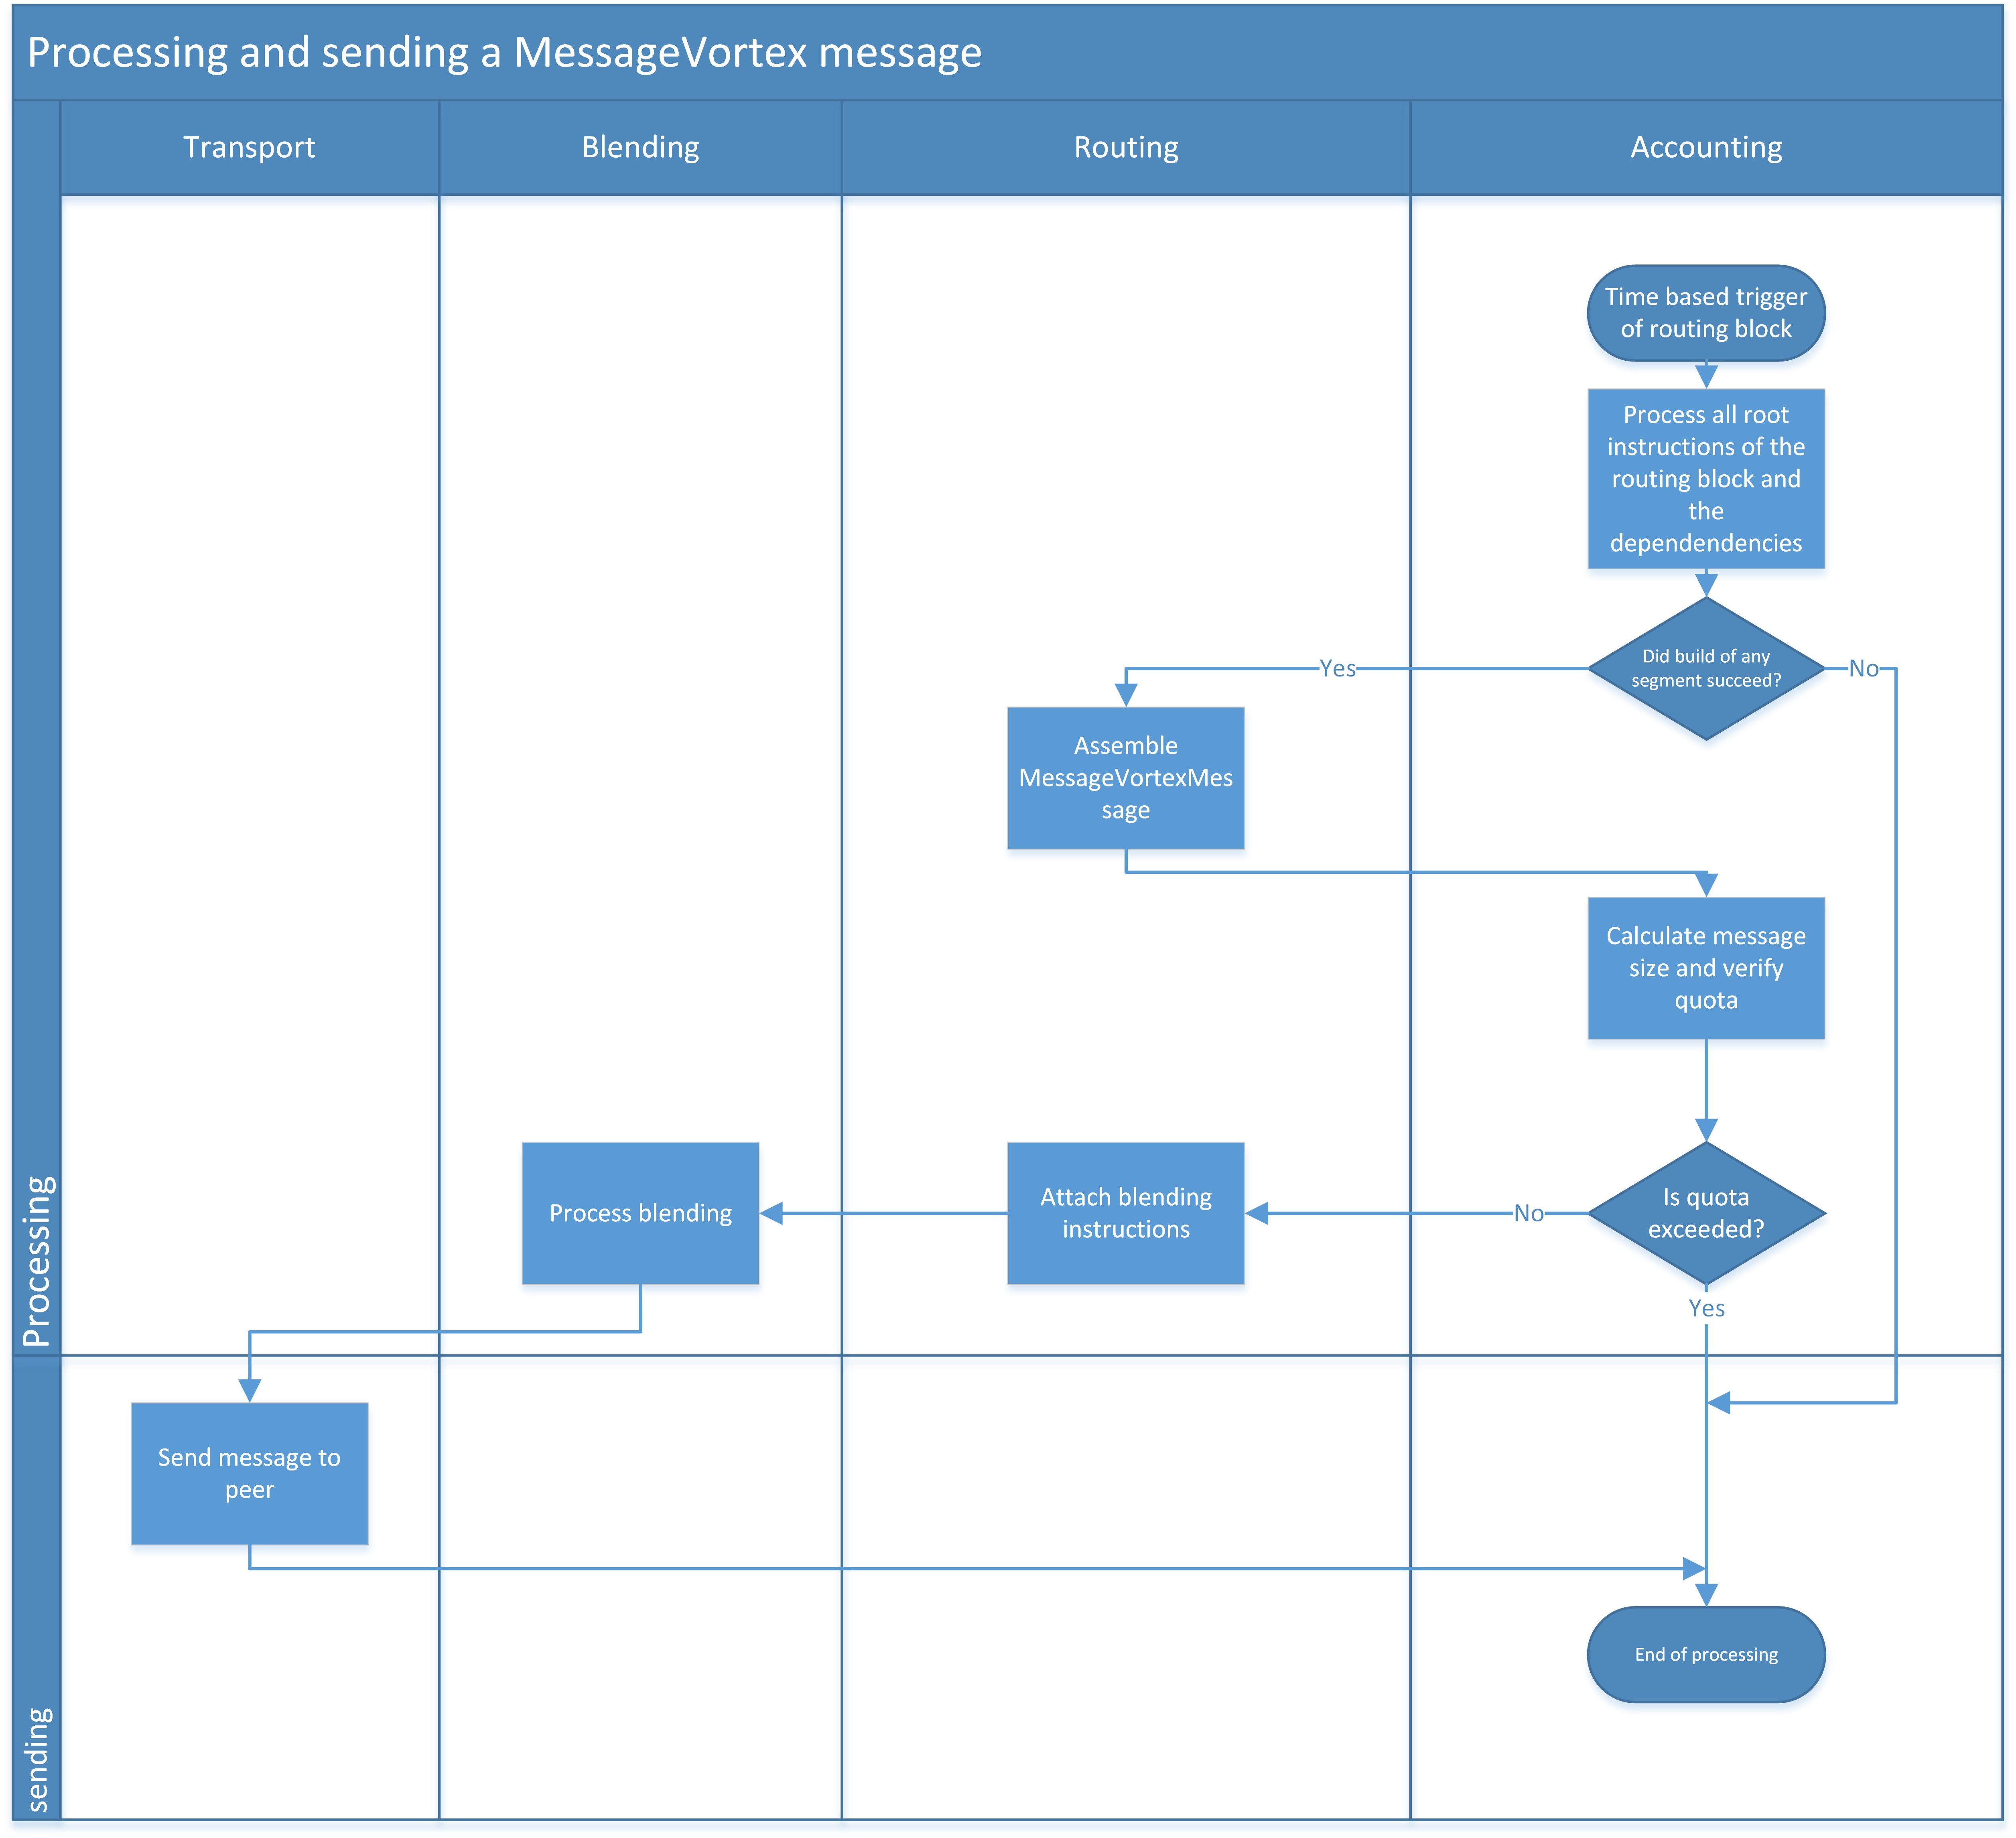
\includegraphics[width=0.90\textwidth]{inc/flowchart_message_sending}
	\caption{flow diagram showing processing of outgoing messages}
	\label{fig:msgSendProcessing}
\end{figure*}

\fxwarning{complete section}

\subsection{Processing of Outgoing Messages}\label{sec:processingOutgoingMessages}
\fxwarning{complete section}

\subsection{Implementation of Operations}\label{sec:implOperations}
\fxwarning{Mention mapping operation}

\fxwarning{Mention floating point issues when splitting}

\fxwarning{complete section}

\section{Request handling}
\fxwarning{complete section}

\subsection{Requesting a new Ephemeral Identity}\label{sec:newEID}
\fxwarning{complete section}

\subsection{Replacing an Existing Node Identity}
\fxwarning{complete section}

\subsection{Replacing an Existing Reply Block}\label{sec:replaceMURB}
\fxwarning{complete section}


\chapter{Accounting Layer Implementation}
\fxwarning{complete section}

\chapter{Usability Related Implementation Details}
\fxwarning{complete section}

\section{Adressing and address representations}
\fxwarning{complete section}

\section{Linking to Common User Agents}
\fxwarning{complete section}

\chapter{Efficiency Related Implementation Details}
\fxwarning{complete section}

\section{Node Storage Management}
\fxwarning{complete section}

\subsection{Life-cycle of Ephemeral Identities and Workspaces}
\fxwarning{complete section}

\subsection{Life-cycle of Requests}
\fxwarning{complete section}

\subsection{Life-cycle of Operations}
\fxwarning{complete section}

\section{Overhead Minimization in Message}
\fxwarning{complete section}


